%===============================================================================
% LaTeX sjabloon voor de bachelorproef toegepaste informatica aan HOGENT
% Meer info op https://github.com/HoGentTIN/latex-hogent-report
%===============================================================================

\documentclass[dutch,dit,thesis]{hogentreport}

% TODO:
% - If necessary, replace the option `dit`' with your own department!
%   Valid entries are dbo, dbt, dgz, dit, dlo, dog, dsa, soa
% - If you write your thesis in English (remark: only possible after getting
%   explicit approval!), remove the option "dutch," or replace with "english".

\usepackage{lipsum} % For blind text, can be removed after adding actual content

%% Pictures to include in the text can be put in the graphics/ folder
\graphicspath{{../graphics/}}

%% For source code highlighting, requires pygments to be installed
%% Compile with the -shell-escape flag!
\usepackage[section]{minted}
%% If you compile with the make_thesis.{bat,sh} script, use the following
%% import instead:
%% \usepackage[section,outputdir=../output]{minted}
\usemintedstyle{solarized-light}
\definecolor{bg}{RGB}{253,246,227} %% Set the background color of the codeframe

%% Change this line to edit the line numbering style:
\renewcommand{\theFancyVerbLine}{\ttfamily\scriptsize\arabic{FancyVerbLine}}

%% Macro definition to load external java source files with \javacode{filename}:
\newmintedfile[javacode]{java}{
    bgcolor=bg,
    fontfamily=tt,
    linenos=true,
    numberblanklines=true,
    numbersep=5pt,
    gobble=0,
    framesep=2mm,
    funcnamehighlighting=true,
    tabsize=4,
    obeytabs=false,
    breaklines=true,
    mathescape=false
    samepage=false,
    showspaces=false,
    showtabs =false,
    texcl=false,
}

% Other packages not already included can be imported here

%%---------- Document metadata -------------------------------------------------
% TODO: Replace this with your own information
\author{Ernst Aarden}
\supervisor{Dhr. F. Van Houte}
\cosupervisor{Mevr. S. Beeckman}
\title[Optionele ondertitel]%
    {Titel van de bachelorproef}
\academicyear{\advance\year by -1 \the\year--\advance\year by 1 \the\year}
\examperiod{1}
\degreesought{\IfLanguageName{dutch}{Professionele bachelor in de toegepaste informatica}{Bachelor of applied computer science}}
\partialthesis{false} %% To display 'in partial fulfilment'
%\institution{Internshipcompany BVBA.}

%% Add global exceptions to the hyphenation here
\hyphenation{back-slash}

%% The bibliography (style and settings are  found in hogentthesis.cls)
\addbibresource{bachproef.bib}            %% Bibliography file
\addbibresource{../voorstel/voorstel.bib} %% Bibliography research proposal
\defbibheading{bibempty}{}

%% Prevent empty pages for right-handed chapter starts in twoside mode
\renewcommand{\cleardoublepage}{\clearpage}

\renewcommand{\arraystretch}{1.2}

%% Content starts here.
\begin{document}

%---------- Front matter -------------------------------------------------------

\frontmatter

\hypersetup{pageanchor=false} %% Disable page numbering references
%% Render a Dutch outer title page if the main language is English
\IfLanguageName{english}{%
    %% If necessary, information can be changed here
    \degreesought{Professionele Bachelor toegepaste informatica}%
    \begin{otherlanguage}{dutch}%
       \maketitle%
    \end{otherlanguage}%
}{}

%% Generates title page content
\maketitle
\hypersetup{pageanchor=true}

%%=============================================================================
%% Voorwoord
%%=============================================================================

\chapter*{\IfLanguageName{dutch}{Woord vooraf}{Preface}}%
\label{ch:voorwoord}

Dit werk is het resultaat van mijn diepgaande interesse en betrokkenheid bij IT-netwerken, die zich ontwikkelde vanaf mijn opleiding in systeembeheer bij VDAB tot mijn huidige rol als netwerkbeheerder binnen het netwerkteam van de \\Universiteit Gent.

Mijn motivatie voor dit onderwerp ontstond uit mijn passie voor IT-netwerken en mijn streven naar een beter begrip van de complexe IT-infrastructuur die onze \\moderne samenleving ondersteunt. 

Met een achtergrond in Cisco-certificeringen en een toewijding aan mijn huidige opleiding Bachelor in de Toegepaste Informatica aan de Hogeschool Gent, zag ik in de uitdagingen van de Universiteit Gent op het gebied van netwerkautomatisering en IP-registratie een kans om mijn kennis en vaardigheden verder te ontwikkelen en toe te passen tijdens mijn studie.

Tijdens mijn onderzoek stuitte ik op verschillende uitdagingen, variërend van het verbeteren van mijn programmeervaardigheden in Python, tot het leiden van een project voor het opzetten van een nieuwe registratietool. Het implementeren van de vereisten van het netwerkteam, met complexe permissies en functionele eisen, bracht zijn eigen uitdagingen met zich mee. Desondanks heb ik deze obstakels met vastberadenheid aangepakt en ben ik gegroeid als professional in het proces.
\\
Ik ben dankbaar voor alle steun die ik heb ontvangen tijdens dit project. Lien en Doesjka verdienen speciale vermelding voor hun onschatbare steun, advies en feedback gedurende de gehele opleiding. Ook wil ik zeker mijn collega en \\copromotor Anne-Mie bedanken voor haar voortdurende begeleiding, advies en haar uitgebreide kennis over IT-netwerken, die van onschatbare waarde was bij het aanpakken van de complexe uitdagingen in dit onderzoek. Verder gaat mijn dank ook uit naar collega Arne voor zijn waardevolle bijdrage aan het project, met name bij het mee nadenken hoe we bepaalde obstakels in de registratietool kunnen oplossen, en zeker ook naar Sion voor zijn rol als promotor, die me steeds heeft voorzien van goede feedback en begeleiding.

Ten slotte hoop ik dat dit werk niet alleen een bijdrage levert aan mijn persoonlijke groei, maar ook aan het begrip en inzicht van de lezer in de complexe wereld van IT-netwerken.

%%=============================================================================
%% Samenvatting
%%=============================================================================

% TODO: De "abstract" of samenvatting is een kernachtige (~ 1 blz. voor een
% thesis) synthese van het document.
%
% Een goede abstract biedt een kernachtig antwoord op volgende vragen:
%
% 1. Waarover gaat de bachelorproef?
% 2. Waarom heb je er over geschreven?
% 3. Hoe heb je het onderzoek uitgevoerd?
% 4. Wat waren de resultaten? Wat blijkt uit je onderzoek?
% 5. Wat betekenen je resultaten? Wat is de relevantie voor het werkveld?
%
% Daarom bestaat een abstract uit volgende componenten:
%
% - inleiding + kaderen thema
% - probleemstelling
% - (centrale) onderzoeksvraag
% - onderzoeksdoelstelling
% - methodologie
% - resultaten (beperk tot de belangrijkste, relevant voor de onderzoeksvraag)
% - conclusies, aanbevelingen, beperkingen
%
% LET OP! Een samenvatting is GEEN voorwoord!

%%---------- Nederlandse samenvatting -----------------------------------------
%
% TODO: Als je je bachelorproef in het Engels schrijft, moet je eerst een
% Nederlandse samenvatting invoegen. Haal daarvoor onderstaande code uit
% commentaar.
% Wie zijn bachelorproef in het Nederlands schrijft, kan dit negeren, de inhoud
% wordt niet in het document ingevoegd.

\IfLanguageName{english}{%
\selectlanguage{dutch}
\chapter*{Samenvatting}
\lipsum[1-4]
\selectlanguage{english}
}{}

%%---------- Samenvatting -----------------------------------------------------
% De samenvatting in de hoofdtaal van het document

\chapter*{\IfLanguageName{dutch}{Samenvatting}{Abstract}}

Het beheren van netwerken en het reserveren van netwerkadressen gebeurt momenteel grotendeels handmatig, wat inefficiënt is als proces, en tevens gevoelig voor menselijke fouten. 

Deze bachelorproef richt zich op het uitwerken van een innovatieve, geautomatiseerde aanpak voor het beheren van netwerken en het
toewijzen van netwerkadressen met behulp van scripts. 
\\Het doel van deze bachelorproef is tweeledig, namelijk (1) het creëren van een tussenlaag van scripts boven een bestaand beheerprogramma voor netwerken, en (2) het nagaan van de impact hiervan op het tijdverbruik voor het toevoegen, wijzigen en verwijderen van nieuwe IP-reserveringen in vergelijking met het huidige handmatige beheerproces. Als resultaat van de bachelorproef kunnen medewerkers via een webpagina die beschikbaar is binnen het bedrijfsnetwerk, mits toestemming van de netwerkbeheerder, eenvoudig netwerkadresreservaties aanmaken, wijzigen of verwijderen.
De webpagina zal de scripts, die binnen het project geschreven worden, aanroepen om de nodige gegevens op de juiste manier aan te leveren aan het beheerprogramma. 

Het verminderen van handmatig beheer van netwerkconfiguraties als resultaat van deze bachelorproef zal leiden tot efficiëntiewinsten, tijdsbesparingen, een vereenvoudigde aanpak en minder fouten. 


%---------- Inhoud, lijst figuren, ... -----------------------------------------

\tableofcontents

% In a list of figures, the complete caption will be included. To prevent this,
% ALWAYS add a short description in the caption!
%
%  \caption[short description]{elaborate description}
%
% If you do, only the short description will be used in the list of figures

\listoffigures

% If you included tables and/or source code listings, uncomment the appropriate
% lines.
%\listoftables
%\listoflistings

% Als je een lijst van afkortingen of termen wil toevoegen, dan hoort die
% hier thuis. Gebruik bijvoorbeeld de ``glossaries'' package.
% https://www.overleaf.com/learn/latex/Glossaries

%---------- Kern ---------------------------------------------------------------

\mainmatter{}

% De eerste hoofdstukken van een bachelorproef zijn meestal een inleiding op
% het onderwerp, literatuurstudie en verantwoording methodologie.
% Aarzel niet om een meer beschrijvende titel aan deze hoofdstukken te geven of
% om bijvoorbeeld de inleiding en/of stand van zaken over meerdere hoofdstukken
% te verspreiden!

%%=============================================================================
%% Inleiding
%%=============================================================================

\chapter{\IfLanguageName{dutch}{Inleiding}{Introduction}}%
\label{ch:inleiding}
In de snel evoluerende wereld van technologie is het doeltreffend beheren van netwerken cruciaal geworden voor het succes van organisaties. Niettemin blijft het handmatig beheren van netwerkconfiguraties, waaronder het toewijzen van specifieke netwerkadressen, een tijdrovend en foutgevoelig proces.

Om deze uitdagingen aan te pakken, zijn er geautomatiseerde netwerkbeheersystemen om het uitdelen van specifieke netwerkadressen te beheren. Een goed uitgewerkt beheersysteem kan een grote meerwaarde bieden voor elk netwerk doordat deze een overzicht kan geven van alle netwerkadressen die in gebruik zijn en hoeveel netwerkadressen er nog beschikbaar zijn per segment van het netwerk.

Dit onderzoek zal scripts voorzien die, via een webportaal en de goedkeuring van netwerkbeheerders, gebruikers zullen toelaten te communiceren met een dergelijk netwerkbeheersysteem om netwerkadres reservaties te maken, te wijzigen of te verwijderen. Dankzij autorisatie zullen gebruikers op het webportaal enkel wijzigingen kunnen aanbrengen voor de netwerken waarvoor de gebruiker gemachtigd is. Nadat de netwerkbeheerder wijzigingen via hetzelfde webportaal goedkeurt, zullen de scripts in werking treden om de nodige aanpassingen binnen het gebruikte beheersysteem te maken.

\section{\IfLanguageName{dutch}{Probleemstelling}{Problem Statement}}%
\label{sec:probleemstelling}
Bij het begin van de bachelorproef worden handmatige registraties van apparaten binnen het netwerk van de Universiteit Gent bijgehouden via tekstbestanden met een vooraf bepaalde structuur. Medewerkers van de Universiteit Gent kunnen via een verouderde webpagina registraties aanmaken voor hun apparaten wanneer dit nodig is. Niet alle medewerkers weten in welk deel van het netwerk de registratie thuishoort, waardoor ze soms enkele belangrijke velden niet kunnen invullen. Indien dit voorkomt, kan het voor de netwerkbeheerder moeilijk zijn om te bepalen in welk netwerksegment de registratie hoort, wat soms tot fouten leidt. Zodra de medewerker de registratie indient, wordt deze als een e-mail naar de netwerkbeheerders gestuurd, die tijd moeten besteden om ervoor te zorgen dat de registratie correct in het juiste tekstbestand wordt geplaatst.

\section{\IfLanguageName{dutch}{Onderzoeksvraag}{Research question}}%
\label{sec:onderzoeksvraag}
Dit onderzoek stelt twee onderzoeksvragen:
\begin{enumerate}
    \item Hoeveel tijd spenderen netwerkbeheerders van Universiteit Gent dagelijks aan het aanmaken, wijzigen en/of verwijderen van manuele netwerkregistraties van toestellen op het netwerk?
    \item Hoe kan men via een softwareportaal van een netwerkbeheersysteem, een eenvoudig te gebruiken platform maken waarop medewerkers van Universiteit Gent netwerkregistraties kunnen aanmaken?
    \begin{enumerate}
        \item Hoe kunnen de netwerkbeheerders van Universiteit Gent registraties via dit platform beheren?
    \end{enumerate}
\end{enumerate}

\section{\IfLanguageName{dutch}{Onderzoeksdoelstelling}{Research objective}}%
\label{sec:onderzoeksdoelstelling}
Deze bachelorproef heeft als doel een webpagina te ontwerpen die via scripts zal communiceren met een nieuw netwerkbeheersysteem. De website biedt medewerkers van de Universiteit Gent de mogelijkheid om informatie van bestaande registraties op te halen, deze te wijzigen of te verwijderen, en nieuwe registraties aan te maken. Na goedkeuring door de netwerkbeheerder van de Universiteit Gent zullen deze registraties op een correcte en veilige manier worden overgebracht naar het nieuwe netwerkbeheersysteem. Daarnaast zal de bachelorproef ook onderzoeken hoeveel tijd kan worden bespaard door het proces van het toevoegen van registraties aan het netwerkbeheersysteem te automatiseren.

\section{\IfLanguageName{dutch}{Opzet van deze bachelorproef}{Structure of this bachelor thesis}}%
\label{sec:opzet-bachelorproef}
De rest van deze bachelorproef is als volgt opgebouwd:

In Hoofdstuk~\ref{ch:stand-van-zaken} wordt een overzicht gegeven van de stand van zaken binnen het onderzoeksdomein, op basis van een literatuurstudie.

In Hoofdstuk~\ref{ch:voorgeschiedenis} wordt het duidelijk welke stappen reeds ondernomen zijn binnen Universiteit Gent in hun migratie naar een nieuw netwerkbeheersysteem.

In Hoofdstuk~\ref{ch:methodologie} wordt de methodologie toegelicht en worden de gebruikte onderzoekstechnieken besproken om een antwoord te kunnen formuleren op de onderzoeksvragen.

In Hoofdstuk~\ref{ch:netadmin-voorbereidingen} wordt beschreven hoe de opbouw en implementatie van de website werd voorbereid om binnen de infrastructuur van Universiteit Gent te passen.

In Hoofdstuk~\ref{ch:netadmin-website-ontwikkeling} worden de belangrijkste onderdelen van de website en hun functie beschreven.

Hoofdstuk~\ref{ch:conclusie}geeft uiteindelijk de conclusie en formuleert een antwoord op de onderzoeksvragen, waarbij ook een aanzet wordt gegeven voor toekomstig onderzoek binnen dit domein.
\chapter{\IfLanguageName{dutch}{Stand van zaken}{State of the art}}%
\label{ch:stand-van-zaken}

% Tip: Begin elk hoofdstuk met een paragraaf inleiding die beschrijft hoe
% dit hoofdstuk past binnen het geheel van de bachelorproef. Geef in het
% bijzonder aan wat de link is met het vorige en volgende hoofdstuk.

% Pas na deze inleidende paragraaf komt de eerste sectiehoofding.

%Dit hoofdstuk bevat je literatuurstudie. De inhoud gaat verder op de inleiding, maar zal het onderwerp van de bachelorproef *diepgaand* uitspitten. De bedoeling is dat de lezer na lezing van dit hoofdstuk helemaal op de hoogte is van de huidige stand van zaken (state-of-the-art) in het onderzoeksdomein. Iemand die niet vertrouwd is met het onderwerp, weet nu voldoende om de rest van het verhaal te kunnen volgen, zonder dat die er nog andere informatie moet over opzoeken \autocite{Pollefliet2011}.

%Je verwijst bij elke bewering die je doet, vakterm die je introduceert, enz.\ naar je bronnen. In \LaTeX{} kan dat met het commando \texttt{$\backslash${textcite\{\}}} of \texttt{$\backslash${autocite\{\}}}. Als argument van het commando geef je de ``sleutel'' van een ``record'' in een bibliografische databank in het Bib\LaTeX{}-formaat (een tekstbestand). Als je expliciet naar de auteur verwijst in de zin (narratieve referentie), gebruik je \texttt{$\backslash${}textcite\{\}}. Soms is de auteursnaam niet expliciet een onderdeel van de zin, dan gebruik je \texttt{$\backslash${}autocite\{\}} (referentie tussen haakjes). Dit gebruik je bv.~bij een citaat, of om in het bijschrift van een overgenomen afbeelding, broncode, tabel, enz. te verwijzen naar de bron. In de volgende paragraaf een voorbeeld van elk.

%\textcite{Knuth1998} schreef een van de standaardwerken over sorteer- en zoekalgoritmen. Experten zijn het erover eens dat cloud computing een interessante opportuniteit vormen, zowel voor gebruikers als voor dienstverleners op vlak van informatietechnologie~\autocite{Creeger2009}.

%Let er ook op: het \texttt{cite}-commando voor de punt, dus binnen de zin. Je verwijst meteen naar een bron in de eerste zin die erop gebaseerd is, dus niet pas op het einde van een paragraaf.

%\lipsum[7-20]
Dit hoofdstuk zal eerst enkele relevante netwerkbegrippen uitleggen en eindigen met gelijkenissen met een gelijkaardig project als deze bachelorproef en wat daaruit kan worden meegenomen.
% TODO: Inleiding stand van zaken


\section{IT Netwerken: fundamenten}
Dit stuk zal enkele fundamentele begrippen uitleggen die binnen elk IT Netwerk belangrijk zijn.

\subsection{IP: Internet Protocol}
% TODO: Bron zoeken om te staven wat ik schrijf over IP
\acrfull{ip} is een set van regels die bepalen hoe een computer data zal versturen naar een andere computer. Het is het fundament van elk gestructureerd, goed functionerend en veilig netwerk. Het maakt efficiënte gegevensoverdracht mogelijk, verdeelt netwerken in beheersbare eenheden, beperkt toegang tot gevoelige informatie of systemen, identificeert services en helpt bij het oplossen van netwerkproblemen \autocite{Postel1981}. Een \acrshort{ip}-adres is volgens \textcite{Postel1981} een belangrijk mechanisme van het \acrshort{ip}. Het is een uniek identificatienummer dat aan elk apparaat is toegewezen, dat verbonden is met een computernetwerk dat het \acrshort{ip} gebruikt voor communicatie. Dit adres helpt andere computers om te weten waar ze informatie naartoe moeten sturen wanneer ze communiceren via een netwerk.
Er zijn twee versies van \acrshort{ip}-adressen, \acrshort{ip}v4 en \acrshort{ip}v6, waarvan de eerste versie bestaat uit vier groepen cijfers gescheiden door punten en de tweede versie uit acht groepen hexadecimale cijfers, gescheiden door dubbele punten. Een octet bestaat uit acht bits, wat betekent dat een octet een bereik heeft van 0 tot 255.

In essentie zorgt een \acrshort{ip}-adres ervoor dat apparaten op het internet met elkaar kunnen communiceren door te weten waar ze gegevens naartoe moeten sturen en waar ze gegevens vandaan kunnen halen.

%Dit hoofdstuk legt uit wat \acrfull{dns} en \acrfull{dhcp} is, waarom \acrshort{ipam} helpt bij het beheren van \acrshort{ip} netwerken en waarom \acrshort{http} nodig is om te communiceren met EIP. 

\subsection{Subnetten}
% TODO: Bron zoeken om te staven wat ik schrijf over IP
Een subnet (kort voor subnetwerk) is een logisch gescheiden deel van een netwerk, het verdeelt een netwerk in kleinere delen voor een efficiënter beheer. Elk subnetwerk bevat een netwerkadres, host-adressen, een broadcastadres en een netwerkmasker. Om dit te verduidelijken wordt hier het netwerk 192.168.0.0/24 ontleed om elk element uit te leggen.

\begin{itemize}
    \item Netwerkadres: Dit is het eerste adres van het netwerk (in het voorbeeld: 192.168.0.0). Dit adres dient om het subnet te identificeren.
    \item Netwerkmasker: Dankzij het netwerkmasker kan worden vastgesteld welk deel (het netwerkgedeelte) van een \acrshort{ip}-adres het netwerk vertegenwoordigt en welk deel (het hostgedeelte) bestemd is voor individuele hosts. In het voorbeeld staat /24, wat aangeeft dat de eerste drie octetten van het \acrshort{ip}-adres het netwerkadres vormen, terwijl het laatste octet beschikbaar is voor apparaten. Dit komt overeen met de notatie 255.255.255.0, waarbij de eerste drie octetten '255' zijn (wat betekent dat ze allemaal voor het netwerk bestemd zijn) en het laatste octet '0' is (wat beschikbaar is voor apparaten). De notatie "/24" komt overeen met drie octetten omdat elk octet in een \acrshort{ip}-adres bestaat uit 8 bits, en "/24" betekent dat er 24 bits worden gebruikt voor het netwerkadres, waardoor er 8 bits overblijven voor de hostadressen.      
    \item Broadcastadres: Dit is steeds het laatste adres van het netwerk (in het voorbeeld: 192.168.0.255). Dankzij dit adres kunnen apparaten berichten sturen naar alle apparaten die zich in dit subnetwerk bevinden.
    \item Hostadressen: Een hostadres is het uniek identificatienummer van een apparaat binnen een subnet. Met behulp van het netwerkmasker kan worden vastgesteld hoeveel hostadressen beschikbaar zijn in elk subnet. In het voorbeeld zijn er 254 beschikbare hostadressen. Het adres 0 wordt gereserveerd voor het netwerkadres en het adres 255 voor het broadcastadres. Dit betekent dat alle adressen tussen 1 en 254 beschikbaar zijn voor apparaten om te gebruiken als hun individuele hostadressen.
\end{itemize}


\acrshort{ip}-netwerken worden door netwerkbeheerders op een logische manier opgesplitst in subnetwerken. Hierbij worden de beschikbare \acrshort{ip}-adressen verdeeld in subnetwerken (subnet). Het eerder beschreven voorbeeldnetwerk 192.168.0.0/24 heeft een hostgedeelte van 256 adressen, waarvan 2 gereserveerd zijn voor het netwerk- en broadcastadres. Dit netwerk zou men bijvoorbeeld kunnen opdelen in twee subnetwerken, netwerk A: 192.168.0.0/25 en netwerk B: 192.168.0.128/25. Deze twee netwerken hebben elk 128 adressen, waarvan ook hier telkens 2 adressen gereserveerd zijn voor het netwerk- en broadcastadres.
Toestellen binnen subnet A zullen elkaar kunnen bereiken terwijl een toestel in een subnet B zonder de nodige routering geen verbinding zal kunnen maken met de toestellen in subnet A.

\section{IT Netwerken: geavanceerde concepten}
Dit stuk zal meer geavanceerde concepten beschrijven die nodig zijn om een netwerk beter te begrijpen en beheren.

\subsection{DNS}
\textcite{Mockapetris1987} schrijft dat \acrshort{dns} een systeem is dat \textit{resource records} gebruikt om onder andere vertalingen te voorzien tussen domeinnamen en \acrshort{ip}-adressen. Een resource record is een gegevenseenheid in de \acrshort{dns}-database die informatie bevat over een specifiek aspect van een domeinnaam. Als voorbeeld kan je via de browser naar google surfen via het \acrshort{ip}-adres \textit{142.251.36.35} of via domeinnaam \textit{www.google.be}. 

Zoals beschreven door \textcite{Mockapetris1987} voorziet \acrshort{dns} meerdere types resource records die netwerkbeheerders kunnen meegeven: 
\begin{itemize}
    \item \textbf{A}: Dit resource record beschrijft een host adres. 
    Vb. \textit{”server1.voorbeeld.com. IN A 192.168.1.1”} maakt de vertaling zodat het toestel met de domeinnaam \textit{server1.voorbeeld.com} bereikbaar is zowel via het \acrshort{ip}-adres \textit{192.168.1.1} als via de domeinnaam. 
    \item \textbf{CNAME}: Dit resource record beschrijft de canonieke naam van een host, het wordt gebruikt om een alias of subdomein naar het hoofddomein door te verwijzen. Vb. \textit{"www.voorbeeld.com. IN CNAME server1.voorbeeld.com"} zorgt dat server1 ook bereikbaar is via "\textit{www.voorbeeld.com}".
    \item \textbf{MX}: Dit resource record is een \textit{mail exchange} record en wordt gebruikt om aan te geven welke mailservers verantwoordelijk zijn voor het ontvangen van mails binnen een domein. Vb. De \acrshort{dns}-server geeft aan dat \textit{”mailserver.\\voorbeeld.com”} de mailserver is door het resource record \textit{"voorbeeld.com. IN MX 10 mailserver.voorbeeld.com"}.
    %Vb. De  \textit{"voorbeeld.com. IN MX 10 mailserver.voorbeeld.com"} geeft de  mee welke server de mailserver is.
    \item \textbf{NS}: Dit resource record is een \textit{name server} record, het beschrijft welke \acrshort{dns}-servers verantwoordelijk zijn voor het beheren van \acrshort{dns}-informatie voor een domein. Vb. \textit{"voorbeeld.com. IN NS dns1.voorbeeld.com"} verwijst naar \textit{dns1} als \acrshort{dns}-server voor het domein “\textit{voorbeeld.com}”.
    \item \textbf{PTR}: Dit resource record is een \textit{Pointer} record, hiermee kan de \acrshort{dns}-server voor een gevraagd \acrshort{ip}-adres de domeinnaam weergeven.
    %het wordt gebruikt om via \acrshort{ip} een vertaling te vragen aan de \acrshort{dns}-server in plaats van via de naam.
    \item \textbf{SOA}: Dit resource record is een \textit{Start of Authority} record die belangrijke informatie bevat over de zone, zoals welke de primaire \acrshort{dns}-server, contactpersonen, etc. zijn.
\end{itemize}

\subsection{DHCP}
Dit protocol voorziet een framework voor het doorgeven van configuratie-informatie naar hosts (lees: computers) op het netwerk . Zo kan een computer bijvoorbeeld een \acrshort{ip}-adres ontvangen waarmee die kan communiceren binnen het netwerk waarop die is aangesloten \autocite{Droms1997}.

Voor \acrshort{dhcp} zullen netwerkbeheerders subnets (of pools van \acrshort{ip}-adressen) aanbieden aan de \acrshort{dhcp}-server. Die zal gebruik maken van deze pools door (onder andere) \acrshort{ip}-adressen uit te delen aan toestellen die verbinden op het netwerk en daarbij de \acrshort{dhcp}-server laten weten dat ze nog geen \acrshort{ip}-adres hebben.

\textcite{Droms1997} schrijft dat \acrshort{dhcp} drie mechanismes gebruikt voor het uitdelen van \acrshort{ip}-adressen:
\begin{itemize}
    \item \textbf{Automatisch}: Permanent toewijzen van een \acrshort{ip}-adres.
    \item \textbf{Dynamisch}: \acrshort{ip}-adres voor een bepaalde tijd toewijzen.
    \item \textbf{Manueel}: Een (door de netwerkbeheerder) vooraf bepaald \acrshort{ip}-adres toewijzen, in vakjargon noemt met dit een \acrshort{ip}-reservatie.
\end{itemize}

\subsection{IPAM}
Naast de vele uitdagingen die zowel \acrshort{dns} als \acrshort{dhcp} met zich meebrengen, is het beheren van de beschikbare \acrshort{ip}-adressen een belangrijk facet in het takenpakket van de netwerkbeheerder. Een slecht beheerd netwerk kan leiden tot \acrshort{ip}-conflicten waarbij meerdere apparaten hetzelfde \acrshort{ip}-adres gebruiken, wat op zijn beurt dan weer kan leiden tot netwerkstoringen en onvoorspelbaar gedrag van apparaten. Daarnaast zou men ook weinig tot geen overzicht hebben van de beschikbare \acrshort{ip}-adressen en subnetten in het netwerk, waardoor het moeilijker is om de beschikbare adressen te beheren en potentiële conflicten te identificeren.

\subsection{DNS, DHCP en IPAM}
De integratie van \acrshort{dns}, \acrshort{dhcp} en \acrshort{ipam} in een enkel systeem wordt vaak aangeduid als \acrshort{ddi}. Dit biedt een benadering voor het beheren van de essentiële netwerkelementen die nodig zijn voor een goed functionerende infrastructuur. Door \acrshort{dns}, \acrshort{dhcp} en \acrshort{ipam} te combineren, kunnen organisaties profiteren van een geïntegreerde aanpak voor het beheer van hun netwerkmiddelen, waardoor efficiëntie en consistentie worden bevorderd. Zoals beschreven door \textcite{Fontein2023}, leggen \acrshort{ddi}-applicaties doorgaans de focus voornamelijk op \acrshort{ipam}. Het zijn toepassingen die de beschikbare \acrshort{ip}-adressen en subnetten op een gestructureerde, overzichtelijke manier weergeven. Doorgaans is \acrshort{ddi} geïntegreerd met de \acrshort{dns}- en \acrshort{dhcp}-servers waardoor men deze componenten vanuit een centrale plek kunnen beheren. Er zijn meerdere \acrshort{ddi}-softwarepakketten ter beschikking die aangeboden worden door bedrijven zoals Solarwinds, Infoblox, en EfficientIP. \acrshort{ugent} heeft ervoor gekozen om \acrlong{eip} aan te schaffen, dus deze bachelorproef zal hier gebruik van maken voor het automatisch beheren van het netwerk.

\subsection{HTTP/HTTPS}
Om communicatie met een \acrshort{api} mogelijk te maken wordt gebruik gemaakt van \acrfull{http}. Dit is een client-serverprotocol die communicatie mogelijk maakt op het Internet. Zoals beschreven door \textcite{Fielding2014} maakt \acrshort{http} gebruik van \acrfull{uri} om unieke web-resources te identificeren en biedt het verschillende methoden \textit{(GET, POST, PUT, DELETE)} waarmee clients acties kunnen uitvoeren op serverresources. \acrshort{http} is \textit{stateless}, elke aanvraag is onafhankelijk, en statuscodes zoals "200 OK"\ en \textit{headers} worden gebruikt om de resultaten en aanvullende informatie van serververzoeken aan te geven, waardoor een gestandaardiseerde communicatie tussen clients en servers mogelijk is.
Om deze informatieoverdracht te beveiligen, wordt \acrfull{https} gebruikt. \acrshort{https} bouwt voort op \acrshort{http}, maar voegt een extra beveiligingslaag toe door middel van \acrshort{ssl}/\acrshort{tls}-encryptie, waardoor de uitwisseling van gegevens tussen client en server wordt versleuteld. Hierdoor worden alle \acrshort{ip}-registraties en andere gegevens beter beschermd tegen potentiële aanvallen.

\section{Gelijkaardig Onderzoek}
In dit onderdeel wordt gekeken naar gelijkaardige projecten waarbij organisaties via scripts hun manueel netwerkbeheer automatiseren via het implementeren van een \acrshort{ddi}-oplossing.

\subsection{VLAN beheer in infoblox}
Zoals beschreven door \textcite{Karaoui2023} hadden ze hun bestaande VLAN-structuur overgezet van excel-bestanden naar \acrshort{ddi} Infoblox. Ze gebruikten python scripts om de \acrshort{api} van de \acrshort{ddi} aan te roepen en de data op de juiste locatie te plaatsen. Hiervoor hadden ze een testomgeving opgezet en hadden ze hun excel-bestanden geconverteerd naar CSV-bestanden. Het voordeel hiervan is dat python een CSV-bestand gemakkelijk kan uitlezen en bewerken aangezien deze steeds een vaste structuur hebben.

Het verschil tussen hun aanpak zal voornamelijk aan de omgeving liggen, \acrshort{ugent} maakt gebruik van back-ups waarbij testen initieel in de productieomgeving van \acrshort{eip} gedaan worden. Aangezien \acrshort{eip} nog niet in productie was werden uitvoerig testen gedaan met het importen en exporteren van alle data, meer info is hierover terug te vinden in \ref{premigratie}.


%%=============================================================================
%% Methodologie
%%=============================================================================

\chapter{\IfLanguageName{dutch}{Methodologie}{Methodology}}%
\label{ch:methodologie}
De methodologie van dit onderzoek is gebaseerd op een gestructureerde aanpak, waarbij gebruik wordt gemaakt van een Agile ontwikkelingsmethodologie. Dit proces is ontworpen om flexibel en iteratief te werken, waardoor aanpassingen en verbeteringen snel kunnen worden doorgevoerd. De verschillende stappen in dit proces worden hieronder beschreven.

\section{Literatuurstudie}
Net zoals bij de meeste onderzoeken begint dit onderzoek met een uitgebreide literatuurstudie. Deze geeft initieel uitleg over enkele belangrijke IT-netwerkconcepten en eindigt met het onderzoeken van vergelijkbare onderzoeken. Deze studie is terug te vinden in hoofdstuk \ref{ch:stand-van-zaken}.

\section{Voorbereidingen}
Na de literatuurstudie werden enkele cruciale voorbereidingen getroffen voordat de ontwikkeling van de nieuwe website van start ging. Deze voorbereidingen omvatten:
\begin{itemize}
    \item \textbf{Metingen van tijdsverbruik}: Er worden metingen gedaan om na te gaan hoeveel tijd netwerkbeheerders van UGent gebruiken om registraties uit te voeren.
    \item \textbf{Flowcharts maken}: Er worden flowcharts gemaakt die de gebruikersacties op de website in kaart brengen. Deze flowcharts helpen bij het visualiseren van de gebruikersinteractie en het structureren van de navigatie en functionaliteit van de website.
    \item \textbf{Infrastructuuronderzoek}: De mogelijkheden worden onderzocht voor het implementeren van de nieuwe website binnen de bestaande infrastructuur van UGent. Hierbij wordt duidelijk dat er een testomgeving met eenvoudig te implementeren apache- en MySQL-servers ter beschikking is.
    \item \textbf{Samenstellen van teamleden}: Er worden collega's aangesproken die kunnen bijdragen aan de ontwikkeling van de front-end. Deze stap zorgt voor een efficiënte verdeling van taken en expertise.
\end{itemize}
Meer gedetailleerde informatie over deze voorbereidingen is te vinden in hoofdstuk \ref{ch:netadmin-voorbereidingen}.

\section{Ontwikkelingsfases}
\label{agile}
De ontwikkelingsfases voor het ontwerpen van de nieuwe registratie-website volgen een Agile aanpak, waarbij er gewerkt wordt in korte, iteratieve sprints. Dit zorgt ervoor dat we snel kunnen reageren op feedback en wijzigingen kunnen doorvoeren. De belangrijkste activiteiten in deze fase zijn:
\begin{itemize}
    \item \textbf{Wekelijkse statusvergaderingen}: Er zijn wekelijkse vergaderingen opgezet met S. Coppens, die verantwoordelijk is voor de back-end ontwikkeling en \\projectoverzicht, met A. De Keyzer, die de front-end ontwikkelt, en met eventuele stakeholders zoals Mevr. A. Vandermeeren die verantwoordelijk is voor de migratie naar EfficientIP. Deze vergaderingen dienen om de voortgang te bespreken, problemen op te lossen en nieuwe ideeën te evalueren.
    \item \textbf{Informeel Contact}: Naast de formele vergaderingen is er regelmatig informeel contact om ideeën uit te wisselen en eventuele wijzigingen in de plannen te bespreken.
\end{itemize}
Deze aanpak wordt gekozen om flexibel, iteratief en efficiënt te zijn, met een sterke focus op samenwerking en voortdurende verbetering. 

\section{Opzetten van testomgeving}
Na de voorbereidingen en de eerste sprint wordt gebruik gemaakt van de testomgeving van UGent, waarin een Apache-server en een MySQL databank opgezet wordt. 
Daarnaast wordt ook in de UGent-Github een repository opgezet waarop de nodige teamleden toegang hebben. GitHub is een webgebaseerd platform voor versiebeheer en samenwerking, waarmee ontwikkelaars code kunnen opslaan, beheren en samen aan projecten kunnen werken met behulp van Git. Het biedt tools voor code review, projectmanagement en integratie met andere ontwikkelingshulpmiddelen.

\section{Database en Automatisering}
Een MySQL-database wordt opgezet in de testomgeving om zowel nieuwe als gewijzigde en verwijderde registraties op te slaan. Deze database dient als tijdelijke opslag tot de wijzigingen worden verwerkt en geüpload naar EfficientIP. Op de Apache-server wordt het script processChanges.py om de zoveel uur automatisch gestart, zodat alle goedgekeurde, onverwerkte wijzigingen worden geüpload naar EfficientIP. Hiermee wordt gestreefd naar een robuuste en gebruiksvriendelijke website die voldoet aan de behoeften van de gebruikers en de infrastructuur van UGent.

Meer informatie over de verschillende versies van de website en de bijbehorende scripts is te vinden in hoofdstuk \ref{ch:netadmin-website-ontwikkeling}.



% Voeg hier je eigen hoofdstukken toe die de ``corpus'' van je bachelorproef
% vormen. De structuur en titels hangen af van je eigen onderzoek. Je kan bv.
% elke fase in je onderzoek in een apart hoofdstuk bespreken.

%\input{...}
%\input{...}
%...

%%=============================================================================
%% Conclusie
%%=============================================================================

\chapter{Conclusie}%
\label{ch:conclusie}
Deze bachelorproef heeft tot doel om de problemen van inefficiëntie en potentiële fouten aan te pakken die ontstaan bij het handmatig beheren van IP-registraties binnen het netwerk van de UGent. Dankzij de ontwikkeling van een nieuwe registratietool, bestaande uit de combinatie van Python-scripts, een gebruiksvriendelijke webinterface, en DDI-systeem EfficientIP, worden aanzienlijke verbeteringen gerealiseerd in termen van efficiëntie, tijdsbesparingen en het verminderen van fouten.
Er wordt een antwoord gegeven op de uitdagingen uit sectie \ref{uitdagingen}:
\begin{itemize}[]
    \item \textbf{Tijd}: Aangezien er een aparte pagina op de registratietool is gemaakt waar netwerkbeheerders de gemaakte registraties of wijzigingen kunnen bekijken en goed- of afkeuren, wat vervolgens automatisch wordt verwerkt, zullen ze tijd besparen. Dankzij de metingen die gedaan zijn in hoofdstuk \ref{ch:netadmin-voorbereidingen} is nu duidelijk dat de netwerkbeheerders hier gemiddeld 17 minuten en 54 seconden per dag zullen besparen.
    \item \textbf{Schaalbaarheid}: EfficientIP stelt UGent in staat om IP-adressen efficiënter toe te wijzen en te beheren, waardoor conflicten worden voorkomen en de uitrol van nieuwe services wordt versneld. Daarnaast automatiseert het routinetaken en ondersteunt het de implementatie van IPv6, waardoor UGent gemakkelijk kan meeschalen met groeiende netwerken en voldoet aan moderne standaarden.
    \item \textbf{Consistentie}: De registratietool maakt het mogelijk voor gebruikers om eenvoudig IP-registraties aan te vragen door middel van een intuïtieve interface. Hierbij wordt de complexiteit van het selecteren van de juiste subnetten verminderd door gebruik te maken van keuzelijsten op basis van campus- en gebouwen, correcte subnetnamen en achterliggende FI-codes. Deze vereenvoudigde aanpak zal potentieel leiden tot minder menselijke fouten. 
    \item \textbf{Beveiliging}: De registratietool houdt bij welke netwerkbeheerder wanneer een registratie heeft goedgekeurd. Deze informatie wordt samen met de goedgekeurde registratie naar EfficientIP verzonden, waardoor altijd bekend is wie de laatste wijziging heeft gedaan. Bovendien wordt alle netwerkdata opgeslagen in een geëncrypteerde database. Dit maakt de de netwerkdata weerbaarder tegen cyberaanvallen, in tegenstelling tot opslag in ongecrypteerde tekstbestanden.
\end{itemize}

\section{Verder onderzoek}
Deze registratietool geeft meerdere mogelijkheden voor verdere verbeteringen, zoals het implementeren van een API voor systeembeheerders, het mogelijk maken van bulkregistraties voor gebruikers, en de implementatie van IPv6.

Dit onderzoek levert een waardevolle bijdrage aan het domein van netwerkbeheer door het ontwikkelen van een innovatieve aanpak voor het beheren en toewijzen van netwerkadressen. Deze aanpak biedt niet alleen tastbare voordelen voor de netwerkbeheerders van UGent, maar heeft ook het potentieel om als model te dienen voor vergelijkbare organisaties die worstelen met vergelijkbare uitdagingen in netwerkbeheer.




%---------- Bijlagen -----------------------------------------------------------

\appendix

\chapter{Onderzoeksvoorstel}

Het onderwerp van deze bachelorproef is gebaseerd op een onderzoeksvoorstel dat vooraf werd beoordeeld door de promotor. Dat voorstel is opgenomen in deze bijlage.

%% TODO: 
%\section*{Samenvatting}

% Kopieer en plak hier de samenvatting (abstract) van je onderzoeksvoorstel.

% Verwijzing naar het bestand met de inhoud van het onderzoeksvoorstel
%---------- Inleiding ---------------------------------------------------------

\graphicspath{ {../voorstel/img/} }

\section{Inleiding}%
\label{voorstel:inleiding}
In de snel evoluerende wereld van technologie is het doeltreffend beheren van netwerken cruciaal geworden voor het succes van organisaties. Echter, het handmatig beheren van netwerkconfiguraties, waaronder het toewijzen van specifieke netwerkadressen, blijft een tijdrovend en foutgevoelig proces.

Om deze uitdagingen aan te pakken, zijn er onder andere geautomatiseerde oplossingen voor Internet Protocol Address Management (IPAM) ontwikkeld. Een goed uitgewerkte IPAM-tool kan een grote meerwaarde bieden voor elk netwerk doordat deze o.a. een overzicht kan geven van alle IP adressen die in gebruik zijn en hoeveel IP adressen er nog beschikbaar zijn per subnet.

Dit onderzoek zal scripts voorzien die, via een webportaal en de goedkeuring van netwerkbeheerders, gebruikers zullen toelaten te communiceren met de IPAM-tool om IP reservaties te maken, wijzigen of verwijderen. Dankzij autorisatie zullen gebruikers op het webportaal enkel wijzigingen kunnen aanbrengen voor de netwerken waarvoor de gebruiker gemachtigd is dit te doen. Nadat de netwerkbeheerder die wijzigingen via hetzelfde webportaal goedkeurt, zullen de scripts in werking treden waarbij de nodige aanpassingen gemaakt worden binnen de gebruikte IPAM-tool.

Het automatisch beheren van IPAM via scripts beoogt niet alleen de efficiëntie van het netwerkbeheer te verhogen, maar ook tijdsbesparingen te realiseren en een meer gestroomlijnde aanpak te bieden. Deze tijdsbesparingen zijn de focus van het onderzoek, waarbij we de volgende onderzoeksvraag trachten te beantwoorden: Hoe beïnvloedt de implementatie van geautomatiseerde scripts het tijdverbruik voor het toevoegen, wijzigen en verwijderen van nieuwe IP-reserveringen in vergelijking met het huidige handmatige beheerproces?

\subsection{Probleemstelling}
\label{voorstel:probleemstelling}
Deze bachelorproef zal uitgevoerd worden bij Universiteit Gent (UGent), directie ICT. Momenteel werkt UGent met scripts die op basis van zogenaamde \textit{subnetbestanden} de nodige acties doen om het netwerk te beheren. 

Deze ongecrypteerde subnetbestanden stellen elk een subnetwerk (een aantal opeenvolgende netwerkadressen) voor en beschrijven cruciale informatie zoals belangrijke naamservers, welk \textit{Virtual Local Area Network (VLAN)} nummer, gateway, etc. Hiernaast bevatten deze zowel alle beschikbare als gereserveerde netwerkadressen met daarbij eventueel enkele regels voor domeinnamen en beveiliging.

Voor elke netwerkadresreservatie die moet gebeuren, vullen geautoriseerde gebruikers via een webportaal alle nodige info in.
Nadat ze deze inzenden stuurt het webportaal een mail naar de groep mailbox van de netwerkbeheerders.
In deze mail zitten dan alle nodige commando's en teksten om de gevraagde wijzigingen aan te brengen aan de relevante subnetbestanden. In sommige gevallen dient de netwerkbeheerder eerst zelf nog uit te zoeken welk subnetbestand nodig is op basis van de documentatie en opzoekwerk. Indien de aanvrager van de reservatie dit heeft meegegeven in een veld voorzien voor commentaar, moet de netwerkbeheerder de eventuele domeinnaam- of beveiligingsregels handmatig toevoegen aan de reservatie.

Het overzicht van de beschikbare subnetwerken is beschreven in een interne wikipediapagina met daarbij de beschrijving van elk subnetwerk. Deze huidige aanpak brengt meerdere uitdagingen met zich mee:
\begin{itemize}
    \item \textbf{Tijd}: Het manueel onderhouden van de scripts, subnetbestanden, netwerkadresreservaties (maken en opkuisen) kan veel tijd vragen. Alle mails met IP registraties moeten elk afzonderlijk bekeken en verwerkt worden.
    \item \textbf{Schaalbaarheid}: Doordat elke wijziging het bestaande bestand overschrijft en er dus geen historische data is kan men moeilijk trends herkennen. Ook wikipediapagina's moet men manueel bijwerken bij grote wijzigingen in de structuur.
    \item \textbf{Consistentie}: De huidige aanpak vraagt meerdere manuele acties, waardoor die vatbaar is voor menselijke fouten of vergissingen. Ook het manueel opzoeken van de relevante subnetbestanden als de aanvrager niet weet in welk subnet de aanvraag terecht moet komen, kan leiden tot registraties in verkeerde subnetten.  
    \item \textbf{Beveiliging}: Zoals beschreven door \textcite{Liao2020} is een van de eerste stappen in een cybersecurity aanval het verzamelen van netwerk informatie via netwerk scan tools zoals Nmap. Het bewaren van alle IP registraties van het volledige domein centraal in cleartext bestanden, zoals nu het geval is, is dan ook een schat aan informatie voor elke individu met al dan niet slechte bedoelingen.
\end{itemize}

UGent is momenteel stappen aan het ondernemen voor het implementeren van \textit{Efficiënt IP (EIP)}, een IPAM-softwarepakket. Dankzij deze implementatie is de verwachting dat de hierboven beschreven indicatoren zullen verbeteren. Om de onderzoeksvraag te beantwoorden zullen er metingen gedaan worden betreffende tijdverbruik. Hierbij zal de huidige manier van werken in tijdsgebruik vergeleken worden met die na de implementatie van het webportaal.

\subsection{Doelstelling}
\label{voorstel:doelstelling}
Deze bachelorproef zal een abstractielaag maken boven EIP waarbij scripts via de \textit{Application Programming Interface (API)} van EIP commando's zullen uitvoeren op EIP.
Door de omvang van het EIP-project is het binnen de voorziene tijd van de bachelorproef niet haalbaar om UGent volledig over te zetten op de werking van EIP. Aangezien dit kritische componenten zijn, zal alles eerst uitvoerig getest worden waarbij elke stap in de migratie naar EIP weloverwogen is.

Daarom stel ik als doel om een eerste versie op te leveren van een webportaal waarop men reeds één of meerdere netwerkadresreservaties kan aanmaken, wijzigen of verwijderen. Aangezien elk subnet specifiek is voor bepaalde verdiepingen, gebouwen en/of vakgroepen, en elke medewerker binnen UGent tot een specifieke vakgroep behoort, zullen we deze informatie gebruiken om te bepalen voor welke relevante subnetten de aanvrager wijzigingen kan aanvragen. Deze aanvragen komen in een duidelijk overzicht terecht waar de netwerkbeheerders al dan niet openstaande reservaties kunnen wijzigen, goedkeuren of weigeren. Na goedkeuring worden de scripts gebruikt om de reservaties toe te passen in EIP.

Dit project geeft een antwoord op de vraag: Hoe kunnen netwerkbeheerders hun werk vereenvoudigen door het gebruik van scripts?
Het beoogde resultaat is:
\begin{itemize}
    \item Het vereenvoudigen van veelvoorkomende taken, zoals het reserveren van internetadressen.
    \item Tijd besparen door het vermijden van handmatige handelingen.
    \item Efficiënter werken door menselijke fouten te voorkomen.
    \item De gebruiksvriendelijkheid verbeteren.
\end{itemize}

Deze verbeteringen zullen helpen bij het optimaliseren van de netwerkinfrastructuur.

\section{Literatuurstudie}
\label{voorstel:begrippen}
Internet Protocol (IP) is het fundament van elk gestructureerd, goed functionerend en veilig netwerk. Het geeft de mogelijkheid efficiënt gegevens te routeren, netwerken te verdelen in meer beheersbare eenheden, toegang te beperken tot gevoelige data of systemen, services te identificeren en het oplossen van netwerkproblemen \autocite{Postel1981}. Dit hoofdstuk legt uit wat \textit{Domain Name System (DNS)} en \textit{Dynamic Host Configuration Protocol (DHCP)} is, waarom IPAM helpt bij het beheren van IP netwerken en waarom HTTP nodig is om te communiceren met EIP. 

\subsection{DNS}
\textcite{Mockapetris1987} schrijft dat DNS een systeem is dat \textit{resource records} gebruikt om onder andere vertalingen te voorzien tussen domeinnamen en IP-adressen. Als voorbeeld kan je via de browser naar google surfen via het IP-adres \textit{142.251.36.35} of via domeinnaam \textit{www.google.be}.

Zoals beschreven door \textcite{Mockapetris1987} voorziet DNS meerdere types resource records die netwerkbeheerders kunnen meegeven: 
\begin{itemize}
    \item \textbf{A}: Dit resource record beschrijft een host adres. 
    Vb. \textit{”server1.voorbeeld.com. IN A 192.168.1.1”} maakt de vertaling zodat het toestel met de domeinnaam \textit{server1.voorbeeld.com} bereikbaar is zowel via het IP-adres \textit{192.168.1.1} als via de domeinnaam. 
    \item \textbf{CNAME}: Dit resource record beschrijft de canonieke naam van een host, het wordt gebruikt om een alias of subdomein naar het hoofddomein door te verwijzen. Vb. \textit{"www.voorbeeld.com. IN CNAME server1.voorbeeld.com"} zorgt dat server1 ook bereikbaar is via "\textit{www.voorbeeld.com}".
    \item \textbf{MX}: Dit resource record is een \textit{mail exchange} record en wordt gebruikt om aan te geven welke mailservers verantwoordelijk zijn voor het ontvangen van mails binnen een domein. vb. \textit{"voorbeeld.com. IN MX 10 mailserver.voorbeeld.com"} geeft de DNS server mee welke server de mailserver is.
    \item \textbf{NS}: Dit resource record is een \textit{name server} record, het beschrijft welke DNS-servers verantwoordelijk zijn voor het beheren van DNS-informatie voor een domein. Vb. \textit{"voorbeeld.com. IN NS dns1.voorbeeld.com"} verwijst naar \textit{dns1} als DNS-server voor het domein “\textit{voorbeeld.com}”.
    \item \textbf{PTR}: Dit resource record is een \textit{Pointer} record, het wordt gebruikt om via IP een vertaling te vragen aan de DNS-server in plaats van via de naam.
    \item \textbf{SOA}: Dit resource record is een \textit{Start of Authority} record die belangrijke informatie bevat over de zone, zoals welke de primaire DNS-server, contactpersonen, etc. zijn.
\end{itemize}

\subsection{DHCP}
Dit protocol voorziet een framework voor het doorgeven van configuratie-informatie naar hosts (lees: computers) op het netwerk . Zo kan een computer bijvoorbeeld een IP-adres ontvangen waarmee die kan communiceren binnen het netwerk waarop die is aangesloten \autocite{Droms1997}.

IP-netwerken worden door netwerkbeheerders op een logische manier opgesplitst in subnetwerken. Hierbij worden de beschikbare IP-adressen verdeeld in subnetwerken (subnet). Toestellen binnen subnet A zullen elkaar kunnen bereiken terwijl een toestel in een subnet B zonder de nodige routering geen verbinding zal kunnen maken met de toestellen in subnet A.

Voor DHCP zullen netwerkbeheerders subnets (of pools van IP-adressen) aanbieden aan de DHCP-server. Die zal gebruik maken van deze pools door (onder andere) IP-adressen uit te delen aan toestellen die verbinden op het netwerk en daarbij de DHCP-server laten weten dat ze nog geen IP-adres hebben.

\textcite{Droms1997} schrijft dat DHCP drie mechanismes gebruikt voor het uitdelen van IP-adressen:
\begin{itemize}
    \item \textbf{Automatisch}: Permanent toewijzen van een IP-adres.
    \item \textbf{Dynamisch}: IP-adres voor een bepaalde tijd toewijzen.
    \item \textbf{Manueel}: Een (door de netwerkbeheerder) vooraf bepaald IP-adres toewijzen, in vakjargon noemt met dit een IP-reservatie.
\end{itemize}

\subsection{IPAM}
Naast de vele uitdagingen die zowel DNS als DHCP met zich meebrengen, is het beheren van de vele DNS records, IP-adres ranges en de vaak vele IP-reservaties zeker iets waar een netwerkbeheerder over moet waken. 
Een mogelijke oplossing hiervoor is het gebruiken van IP Address Management (IPAM) via softwarepakketten die IPAM aanbieden.
IPAM laat toe IP-adressen efficiënt te beheren in een netwerk, het leidt tot een gestructureerde aanpak waardoor conflicten tussen subnetten worden vermeden. Het geeft een compleet overzicht van het netwerk met percentages van hoeveel adressen beschikbaar en in gebruik zijn. IPAM geeft eveneens de mogelijkheid om de historiek bij te houden waardoor het van pas komt voor schaalbaarheid en beveiliging van het netwerk \autocite{Rooney2020}.

\subsection{HTTP/HTTPS}
Om communicatie met de API van EIP mogelijk te maken wordt er gebruik gemaakt van \textit{Hypertext Transfer Protocol (HTTP)}. Dit is een client-serverprotocol die communicatie mogelijk maakt op het Internet. Zoals beschreven door \textcite{Fielding2014} maakt HTTP gebruik van \textit{Uniform Resource Identifiers (URI's)} om unieke web-resources te identificeren en biedt het verschillende methoden \textit{(GET, POST, PUT, DELETE)} waarmee clients acties kunnen uitvoeren op serverresources. HTTP is \textit{stateless}, elke aanvraag is onafhankelijk, en statuscodes zoals "200 OK"\ en \textit{headers} worden gebruikt om de resultaten en aanvullende informatie van serververzoeken aan te geven, waardoor een gestandaardiseerde communicatie tussen clients en servers mogelijk is.
Om deze informatieoverdracht te beveiligen, wordt \textit{Hypertext Transfer Protocol Secure (HTTPS)} gebruikt. HTTPS bouwt voort op HTTP, maar voegt een extra beveiligingslaag toe door middel van \textit{Secure Sockets Layer (SSL)/Transport Layer Security (TLS)}-encryptie, waardoor de uitwisseling van gegevens tussen client en server wordt versleuteld. Hierdoor worden alle IP-registraties en andere gegevens beter beschermd tegen potentiële aanvallen.

\section{Methodologie}
\label{voorstel:methodologie}
In dit hoofdstuk wordt beschreven hoe lang en hoe de nodige metrics voor de onderzoeksvraag worden opgemeten, welke software het project gebruikt, hoe deze worden toegepast, en welke fases het project zal doorlopen.

\subsection{Software}
Alle scripts worden geschreven in \textbf{Visual studio code} in de programmeertaal \textbf{Python}.
Om de HTTP methodes naar de API van EIP te testen, wordt er gebruik gemaakt van \textbf{Postman}.
\begin{itemize}
    \item \textbf{Visual Studio Code}: Vanwege de ondersteuning voor meerdere programmeer- en scripttalen, geïntegreerde Git-ondersteuning, debug- en extensie mogelijkheden wordt gekozen om alle scripts in Visual Studio Code te schrijven.
    \item \textbf{Python}: \textcite{VanRossum2011} beschrijven Python als een eenvoudige, doch krachtige programmeertaal. De beschikbaarheid van Python-pakketten zoals ’requests’ maakt het mogelijk om efficiënt gegevens door te sturen naar API’s zoals die van EIP. Als interpretatieve taal biedt Python snelle ontwikkeling zonder de noodzaak van compilatie. Python is ook uitbreidbaar, waardoor het eenvoudig is om nieuwe functies toe te voegen. Kortom, Python, met zijn netwerkbibliotheken, vormt een ideale keuze voor dit onderzoeksproject \autocite{VanRossum2011}.
    \item \textbf{Postman}: Dit programma geeft de mogelijkheid alle HTTP-verzoeken manueel te maken, versturen en ontvangen. Hierbij is het mogelijk om alle onderdelen van het verzoek te manipuleren en na te gaan wat als resultaat verwacht kan worden bij het uitsturen van bepaalde verzoeken naar de API.
\end{itemize}

\subsection{Methodiek scripts}
Voordat een script wordt geschreven, worden eerst gerichte testen gedaan waarbij commando's met parameters naar de API van EIP worden verzonden. Hierbij wordt er zowel naar de resultaten van de API gekeken als naar wat er op EIP zelf gebeurt via de webpagina. Eens deze testen voor een commando afgelopen zijn, wordt er pas overgegaan tot het schrijven van het Python-script. Hierbij worden telkens de parameters binnen elk script opgezet volgens de voorwaarden van de API.

\subsection{Fase 1. Pre-analyse}
In de eerste fase van de bachelorproef worden er dagelijks metingen gedaan om na te gaan hoeveel tijd een netwerkbeheerder van UGent gebruikt om IP reservaties aan te maken, te wijzigen en/of te verwijderen. Hierbij wordt voor elk type actie de tijd afzonderlijk gemeten en beschreven in een spreadsheet die als bijlage aan het onderzoek wordt toegevoegd.

\subsection{Fase 2. Literatuurstudie}
Voor deze tweede fase worden veertien dagen uitgetrokken. In deze fase wordt gezocht naar documentatie en literatuur van gelijkaardige projecten waarbij een webpagina met formulieren en logins gebruiken om scripts aan te roepen. Daarnaast wordt er ook uitgebreid aandacht gegeven aan de literatuur van Efficiënt IP zelf om na te gaan welke eisen deze stelt voor het aanmaken, wijzigen en verwijderen van IP-adressen.
Op het einde van deze fase zal er een verslag geschreven worden met alle belangrijke punten die zijn meegenomen uit de literatuur.

\subsection{Fase 3. Scripts schrijven}
Binnen de derde fase wordt het grootste stuk van de Python-scripts geschreven. Deze fase voorziet telkens één week om een script te schrijven en daarop aansluitend één week om het geschreven script te testen en te troubleshooten. De drie scripts zijn:
\begin{itemize}
    \item Maken van een IP reservatie
    \item Wijzigen van een bestaande IP reservatie
    \item Verwijderen van een bestaande IP reservatie
\end{itemize}

\subsection{Fase 4. Webpagina schrijven}
Het schrijven van de webpagina begint halverwege fase twee aangezien deze nauw op elkaar aansluiten.
Voor het schrijven van de hoofdpagina van waar de drie scripts kunnen worden aangeroepen, worden drie weken voorzien. Hierna zijn er nog drie weken voorzien voor het schrijven van de netwerkbeheerderspagina. Op deze pagina kan de netwerkbeheerder de gevraagde wijzigingen nakijken, aanpassen en goed- of afkeuren. 

\subsection{Fase 5. Post-analyse}
Tijdens deze laatste fase worden er opnieuw metingen gedaan om na te gaan hoeveel tijd de netwerkbeheerders van UGent nodig hebben voor elke afzonderlijke registratie. Ook in deze fase zullen de metingen in een spreadsheet komen om de nodige vergelijkingen te maken met de data uit de eerste fase van de bachelorproef.

\subsection{Gantt stappenplan}
Een overzicht van alle fases worden weergegeven in dit Gantt stappenplan
\begin{figure}[h!]
    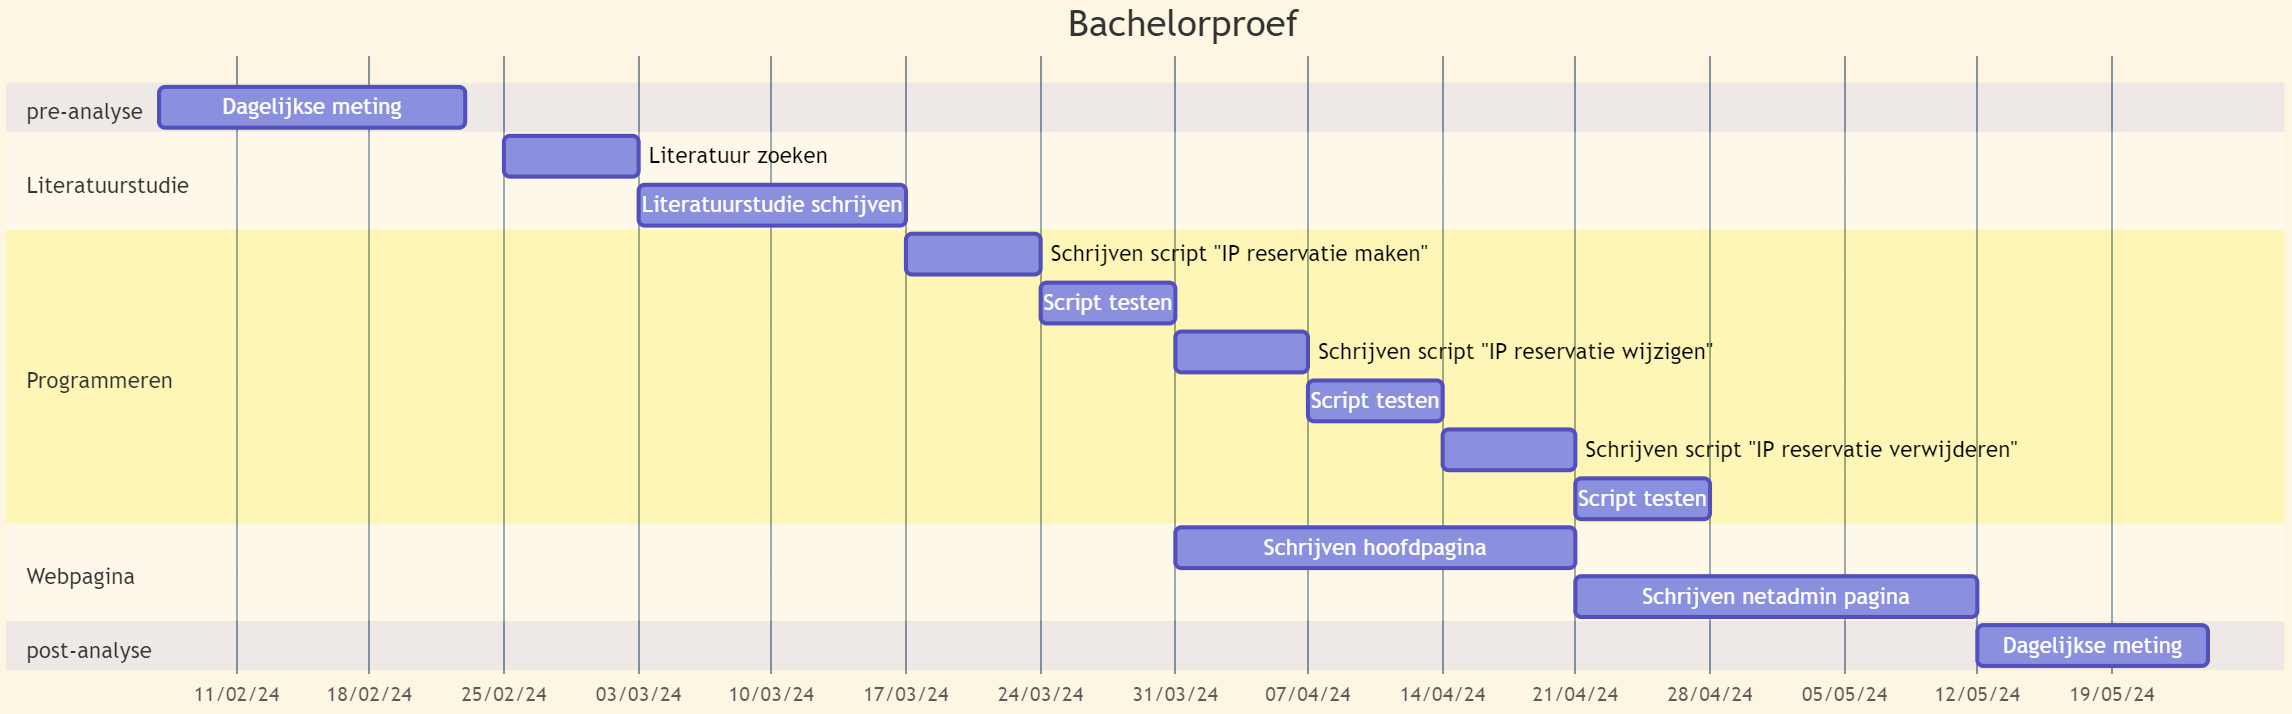
\includegraphics[scale=0.39]{Gantt}
    \caption{Gantt Stappenplan}
    \label{Gantt Stappenplan}
\end{figure}

% Refereren naar de literatuur kan met:
% \autocite{BIBTEXKEY} -> (Auteur, jaartal)
% \textcite{BIBTEXKEY} -> Auteur (jaartal)
% Voorbeeld van een referentie waar de auteursnaam geen onderdeel van de zin is~\autocite{Moore2002}.

\section{Verwachte resultaten}
\label{voorstel:verwachte-resultaten}
% TODO: (fase 6) beschrijf wat je verwacht uit je onderzoek en waarom (bv. volgens je literatuuronderzoek is softwarepakket A het meest gebruikte en denk je dat het voor deze casus ook het meest geschikt zal zijn). Natuurlijk kan je niet in de toekomst kijken en mag je geen alternatieve mogelijkheden uitsluiten. In de praktijk gebeurt het ook vaak dat een onderzoek tot verrassende resultaten leidt, dat maakt het proces nog interessanter!
De verwachte resultaten omvatten een succesvolle eerste implementatie van een webportaal waarop men reeds één of meerdere netwerkadresreservaties kan aanmaken, wijzigen of verwijderen. Deze eerste versie van het intuïtieve webportaal zou een verbeterde gebruikerservaring moeten bieden door middel van geoptimaliseerde API-aanroepen. Verder zou de automatisering van netwerkconfiguraties, met name IP-adresallocatie, moeten leiden tot verminderde complexiteit, verbeterde efficiëntie en algemene gebruiksvriendelijkheid in het netwerkbeheerproces. Dit zal een belangrijke stap zijn om na het project op voort te bouwen om uiteindelijk een product op te leveren.


\section{Verwachte conclusie}
\label{voorstel:discussie-conclusie}
Dankzij het implementeren van deze webpagina met de onderliggende scripts, kunnen medewerkers van Universiteit Gent eenvoudig, consistent, en snel IP-reservaties maken, wijzigen en verwijderen. De netwerkbeheerders kunnen al deze wijzigingen dan op hun eigen webpagina controleren, aanpassen en beoordelen.
Na dit onderzoek zullen er nog voldoende mogelijkheden zijn om de webpagina aan te vullen met extra functies, in die mate dat netwerkbeheerders zelf geen wijzigingen meer dienen te maken binnen de IPAM tool zelf.

%------------------------------------------------------------------------------
% Referentielijst
%------------------------------------------------------------------------------
% TODO: (fase 4) de gerefereerde werken moeten in BibTeX-bestand
% bibliografie.bib voorkomen. Gebruik JabRef om je bibliografie bij te
% houden.

%\printbibliography[heading=bibintoc]

%\end{document}

%%---------- Andere bijlagen --------------------------------------------------
% TODO: Voeg hier eventuele andere bijlagen toe. Bv. als je deze BP voor de
% tweede keer indient, een overzicht van de verbeteringen t.o.v. het origineel.
%\input{...}

%%---------- Backmatter, referentielijst ---------------------------------------

\backmatter{}

\setlength\bibitemsep{2pt} %% Add Some space between the bibliograpy entries
\printbibliography[heading=bibintoc]

\end{document}
